\scanpage{5}
\mspage{3}
\margin{\figure{\begin{tikzpicture}\draw (0,0)--(.6,-.65);\end{tikzpicture}}}

\noindent\textcircled{3}\quad
\uline{pg23}\quad On peut dire plus simplement que ${}_nK$ est étale séparé car ${}_nK=\operatorname{Ker}({}_nG\longrightarrow{}_nH)$. En a), ne dirais-tu pas que ${}_nK_{\bar s}$ est isomorphe à un sous-groupe de ${}_nK_{\bar t}$.

\noindent\uline{pg24}\quad a) $\ell\,15$ :\quad
\begingroup\setbox0=\hbox{$\dim$}\hbox{\rlap{
\begin{tikzpicture}[overlay,baseline=0pt]\draw[gray,line width=.35pt] (3pt,15pt) .. controls (-10pt,11pt) and (-7pt,-6pt) .. (8pt,-7pt) .. controls (\dimexpr\wd0+14pt\relax,-7pt) and (\dimexpr\wd0+15pt\relax,17pt) .. (\dimexpr\wd0-1pt\relax,18pt);\end{tikzpicture}}\box0}\endgroup$\operatorname{Ker}(u_\eta)=0$\quad ?

\noindent\rlap{
\begin{tikzpicture}[overlay,baseline]
\draw (0.62,.65) .. controls (-.15,.63) and (-.45,.08) .. (-.22,-.54) .. controls (.04,-1.03) and (.95,-.59) .. (1.02,.11) .. controls (1.05,.47) and (.84,.68) .. (.62,.65);
\draw[gray] (-.17,.47) .. controls (-.42,.13) and (-.27,-.05) .. (.1,-.03);
\end{tikzpicture}}
\uline{pg28}\quad Les notions introduites dans 3.5 ont elles été définies pour $S$ non hensélien ? (il faudrait au moins choisir un groupe d'inertie).
\inserted{[\unsure{itou|item} pour 3.7]}

\noindent\uline{pg29}\quad $\ell-2$\quad la terminologie ``clôture normale'' est-elle encore canonique ?

\figure{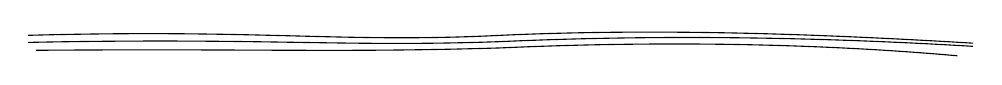
\begin{tikzpicture}
\draw (0,0) .. controls (3,.08) and (4,-.1) .. (6,0) .. controls (8,.09) and (10,.02) .. (12,-.1);
\draw (0,-.09) .. controls (3,-.03) and (4,-.15) .. (6,-.08) .. controls (8,.01) and (10,-.02) .. (12,-.14);
\draw (.1,-.19) .. controls (3,-.17) and (4,-.22) .. (6,-.16) .. controls (8,-.07) and (10,-.1) .. (11.8,-.26);
\end{tikzpicture}}

\noindent\textcircled{4}\quad
\uline{p32}\quad $\ell\,8$\quad ne dépend
\begingroup\setbox0=\hbox{pas}\hbox{\rlap{\begin{tikzpicture}[overlay,baseline=0pt]\draw[gray,line width=.35pt] (\dimexpr\wd0+2pt\relax,15pt) .. controls (-10pt,20pt) and (-8pt,-8pt) .. (3pt,-8pt) .. controls (\dimexpr\wd0+12pt\relax,-8pt) and (\dimexpr\wd0+10pt\relax,8pt) .. (\dimexpr\wd0+5pt\relax,13pt);\end{tikzpicture}}\box0}\endgroup

\noindent\rlap{\begin{tikzpicture}[overlay,baseline]
\draw (1.1,.28) .. controls (.83,.83) and (-1.0,.46) .. (-1.65,-.25) .. controls (-2,-.95) and (-1.15,-1.44) .. (-.22,-1.29) .. controls (.72,-1.15) and (1.33,-.3) .. (1.17,.2);
\end{tikzpicture}}
\makebox[0pt][r]{\raisebox{-.5ex}{\Large ?}\hspace{1.5em}}\uline{pg33 ss}\quad
(4.2)\quad Ne donnerais tu pas un énoncé style ``voisinage tubulaire'' compréhensible. La vérité est

\deleted{\illegible{1}} on a un morphisme de topos $\operatorname{Spec}(K)_{\mathrm{et}}\xrightarrow{\varphi}\operatorname{Spec}(k)_{\mathrm{et}}$ (``\unsure{ext.|ent.} du corps résiduel'') et $A_0^0$ est un schéma relatif sur $(\operatorname{Spec}(K))_{\mathrm{et}}$ annelé par $\varphi^*\mathcal O$ [le $\varphi^*$ des faisceaux d'ensembles] - Même chose d'ailleurs pour
\[
\begin{array}[t]{c}\text{lim}\\[-.8ex]\longrightarrow\\[-.6ex]\text{ramifier.}\end{array}\;A_0
\]

\noindent\rlap{\begin{tikzpicture}[overlay,baseline]\draw[rotate=23] (-.15,-.1) ellipse (1.35 and .52);\end{tikzpicture}}
\makebox[0pt][r]{\raisebox{-.8ex}{\unsure{si} ?}\hspace{1.5em}}\uline{pg36}\quad
$\ell-6$.\quad ``ce n'est pas la trace qui est contragrédiente; l'énoncé primitif était correct -

\noindent\uline{pg40}\quad (4.5.4)\quad Qu'est-il écrit dans la marge ?

$\ell-1$\quad Quel est loc cit. ?

$\ell\,3$\quad $\ell$-groupe signifie-t-il tué par $\ell$, ou par un $\ell^k$ ?

le \unsure{trait|tout} est-il strictement local ? ce serait plus agréable.

\margin{4}
